%% LaTeX-Beamer template for KIT design
%% by Erik Burger, Christian Hammer
%% title picture by Klaus Krogmann
%%
%% version 2.1
%%
%% mostly compatible to KIT corporate design v2.0
%% http://intranet.kit.edu/gestaltungsrichtlinien.php
%%
%% Problems, bugs and comments to
%% burger@kit.edu

\documentclass[18pt]{beamer}

%% SLIDE FORMAT

% use 'beamerthemekit' for standard 4:3 ratio
% for widescreen slides (16:9), use 'beamerthemekitwide'
\usepackage{listings}
\usepackage{templates/beamerthemekit}
% \usepackage{templates/beamerthemekitwide}

%% TITLE PICTURE

% if a custom picture is to be used on the title page, copy it into the 'logos'
% directory, in the line below, replace 'mypicture' with the 
% filename (without extension) and uncomment the following line
% (picture proportions: 63 : 20 for standard, 169 : 40 for wide
% *.eps format if you use latex+dvips+ps2pdf, 
% *.jpg/*.png/*.pdf if you use pdflatex)

\titleimage{logologo}

%% TITLE LOGO

% for a custom logo on the front page, copy your file into the 'logos'
% directory, insert the filename in the line below and uncomment it

%\titlelogo{mylogo}

% (*.eps format if you use latex+dvips+ps2pdf,
% *.jpg/*.png/*.pdf if you use pdflatex)

%% TikZ INTEGRATION

% use these packages for PCM symbols and UML classes
% \usepackage{templates/tikzkit}
% \usepackage{templates/tikzuml}

% the presentation starts here

\title[Short title]{Mathe-1}
%\subtitle{Something for XYZ 2009}
\author{Charlotte P., Lena W., Vera C., Christian K.}

\institute{ITI Wagner \& IPD Tichy}

% Bibliography

\usepackage[citestyle=authoryear,bibstyle=numeric,hyperref,backend=biber]{biblatex}
\addbibresource{templates/example.bib}
\bibhang1em

\begin{document}

% change the following line to "ngerman" for German style date and logos
\selectlanguage{ngerman}

%title page
\begin{frame}
\titlepage
\end{frame}

%table of contents
\begin{frame}{Gliederung}
\tableofcontents
\end{frame}

\section {Big Integer}
\begin{frame}{Big integer}
\begin {itemize}
\item die maximale Zahl ist gr"o"ser als integer?
\pause 
\item nehme long long
\pause
\item die Zahl ist gr"o"ser als long long
\pause 
\item ?????????????????????????????????? (Panik) 
\end {itemize}
\end{frame}

\begin{frame}{Big integer - Java nutzen}
\begin {itemize}
\item import java.math.BigInteger
\item Konstruktor: BigInteger(String val)
\item Methoden:
\begin {itemize}
\item BigInteger add(BigInteger val)
\item BigInteger multiply(BigInteger val)
\item BigInteger subtract(BigInteger val)
\item ...
\end {itemize}
\end {itemize}
\end{frame}

\begin{frame} {Laufzeiten}
\begin {itemize}
\item Addition, Subtraktion in $\mathcal{O}(n)$
\item Multiplikation in $\Theta(n^{log_{2}3})$ (Karatsuba)
\end {itemize}
\end{frame}


\begin{frame} {C++? Selbst implementieren!}
\begin {itemize}
\item Addition: Die Tafel ist da $\longrightarrow{}$
\item Multiplikation (z.B. Karazuba-Multiplikation)
\end {itemize}
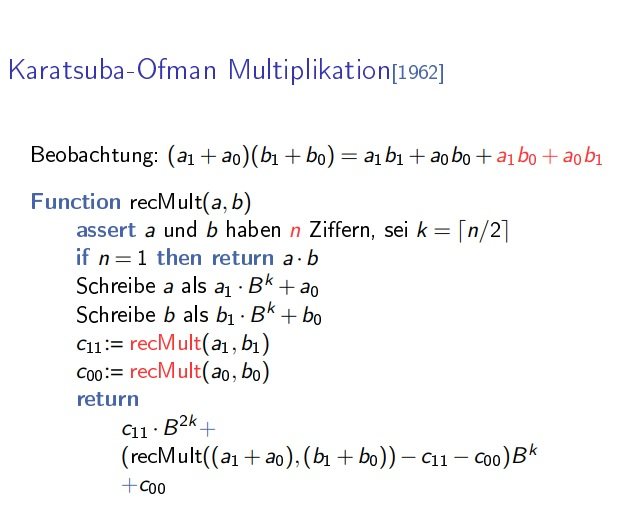
\includegraphics[scale=0.4]{karatsuba.jpg}
\end{frame}

\section {Exponentiation by squaring}
\begin{frame} {Naive Exponentiation} 
\lstinputlisting[language=c++]{exp.cpp}
Bei ICPC gehen wir davon aus, dass Multiplikation zweier Zahlen in $\mathcal{O}(1)$ liegt, also naive Exponentiation in $\mathcal{O}(n)$
\end{frame}

\begin{frame} {Idee}
Beobachtung:
\begin{equation}
   x^{n} =
   \begin{cases}
     (x^{2})^{n/2} & \text{f"ur n gerade} \\
      x*(x^{2})^{(n-1)/2} & \text{f"ur n ungerade} \\
   \end{cases}
\end{equation}
\end{frame}

\begin{frame} {Exponentiation by squaring, rekursive Implementierung}
\lstinputlisting[language=c++]{recExpSq.cpp}
\end{frame}

\begin{frame} {Exponentiation by squaring, iterative Implementierung}
\lstinputlisting[language=c++, basicstyle=\tiny]{iterExpSq.cpp}
Da Multiplikation konstant viel Zeit ben"otigt, liegt die Exponentiation$\mathcal{O}(log(n))$
\end{frame}


\begin{frame}{Hier kommt ein kleines Beispiel auf dem Tafel}
\end{frame}


\section{Section 1}
\subsection{Subsection 1.1}
\begin{frame}{Example slide A}
\begin{itemize}
\item PCM, Citation: \cite{becker2008a} %\language
\pause
\item Bullet point 2
\item \dots
\end{itemize}
\end{frame}

\subsection{Subsection 1.2}
\begin{frame}{Example slide B}
\begin{block}{Block 1}
\begin{itemize}
\item Bullet point 1
\pause
\item Bullet point 2
\item \dots
\end{itemize}
\end{block}
\end{frame}

\section{Section 2}
\begin{frame}{Example slide C}
\begin{exampleblock}{Example 1}
\begin{itemize}
\item Bullet point 1
\pause
\item Bullet point 2
\item \dots
\end{itemize}
\end{exampleblock}
\end{frame}

\begin{frame}{Example slide D}
\begin{alertblock}{Alert 1}
\begin{itemize}
\item Bullet point 1
\pause
\item Bullet point 2
\item \dots
\end{itemize}
\end{alertblock}
\end{frame}

\appendix
\beginbackup

\begin{frame}[allowframebreaks]{References}
\printbibliography
\end{frame}

\backupend

\end{document}
